\section{Convergence, Timestep, and Tolerance}

The program is designed to be called from a command line interface and takes four arguments:
\begin{enumerate}
    \item The stopping criterion.
    \item The Reynolds number.
    \item The timestep $\Delta t$.
    \item The density of the mesh $N$.
\end{enumerate}
Each of these four arguments has a major impact on the outcome of the simulation and must therefore be considered. 

The simulation will halt when
\begin{equation}
    \frac{ \text{max} \left( \left| \mathbf{u}^n - \mathbf{u}^{n-1} \right| \right) }{\Delta t} < \text{tolerance}
\end{equation}
where the tolerance is the stopping criterion to be supplied as a command line argument. A tolerance of $1 \cdot 10^{-5}$ turned out to be good compromise between accurate results and a reasonable execution time. The Reynolds number was fixed at 1000 to match the Reynolds number used to generate the benchmark results. The mesh density $N$ was increased from 16 to 96 with four intermediate steps. The timestep $\Delta t$ is highly dependent on the mesh density $N$. In some numerical methods, it is crucial to choose the timestep such that the flow does not cover a distance larger than the smallest mesh spacing within one period $\Delta t$. This is known as the Courant–Friedrichs–Lewy (CFL) condition:
\begin{equation}
    C = \frac{u \Delta t}{\Delta x} \leq C_{\text{max}}
\end{equation}
where $C_{\text{max}}$ is typically 1, so
\begin{equation}
    \Delta t \leq \frac{C_{\text{max}} \Delta x}{u}
\end{equation}
While the CFL condition is not a necessary nor sufficient condition for convergence, it can definitely serve as a guideline. The CFL condition turned out to hold within an order of magnitude. The final value of $\Delta t$ was determined by trial and error. A timestep that is too large will cause the solution to diverge and a timestep too small will cause slow convergence. The optimal timestep is some value just shy of the value that would cause the solution to diverge. The parameters that were used in the generation of the final results are tabulated in Table \ref{tab:results2}.

\begin{table}[h]
    \centering
    \begin{tabular}{rrrrrrr}  
        \toprule
        \# & $N$ & $\Delta t$ & tolerance & Re & iterations & $\text{iterations} \cdot \Delta t$ \\
        \midrule
        1 & 16 & 0.05 & $1 \cdot 10^{-5}$ & 1000 & ? & ? \\
        2 & 32 & 0.004 & $1 \cdot 10^{-5}$ & 1000 & ? & ? \\
        3 & 48 & ? & $1 \cdot 10^{-5}$ & 1000 & ? & ? \\
        4 & 56 & ? & $1 \cdot 10^{-5}$ & 1000 & ? & ? \\
        5 & 64 & 0.0002 & $1 \cdot 10^{-5}$ & 1000 & ? & ? \\
        6 & 96 & 0.000048 & $1 \cdot 10^{-5}$ & 1000 & ? & ? \\
        \bottomrule
    \end{tabular}
    \caption{Settings for different runs of the simulation.}
    \label{tab:results2} 
\end{table}


\section{Stream Function}

The stream function $\tilde{\psi}$ is defined such that the difference $\Delta \tilde{\psi}$ between two streamlines is equal to the mass flux between two streamlines. This fact allows us to compute the stream function based on the values of flux along the line segments. The outer-oriented line segments $\tilde{u}_{i,j}$ and $\tilde{v}_{i,j}$ represent flux in the form:
\begin{flalign}
    \stepcounter{equation}
    \tag{{\theequation}a}
    \label{eq:results1}
    & & \tilde{u}_{i,j} = \int_{y_{i,j}}^{y_{i,j+1}} \mathbf{u} \cdot  \mathbf{\hat{n}} \, dy && \\
    \tag{{\theequation}b}
    \label{eq:results2}
    &\text{and}& \tilde{v}_{i,j} = \int_{x_{i,j}}^{x_{i+1,j}} \mathbf{u} \cdot \mathbf{\hat{n}} \, dx &&
\end{flalign}
where $\mathbf{\hat{n}}$ denotes the normal vector along the line segment. Thus, computing the stream function is a simply matter of assuming that the stream function has a value of zero at the boundaries and using either Equation \eqref{eq:results1} or Equation \eqref{eq:results2} to compute the unknowns.

Figure \ref{fig:SFN64} shows a contour plot of the stream function for $N = 64$, $\text{Re} = 1000$, $\Delta t = 0.0002$, and $\text{tol} = 1 \cdot 10^{-5}$. Figure \ref{fig:benchmarkSFN64} shows the benchmark result from \parencite{botella1998benchmark}. The contour levels associated with the labels $a$--$j$ in Figure \ref{fig:benchmarkSFN64} can be found in Table 7 of \parencite{botella1998benchmark}. The two figures are, for all intents and purposes, identical. 

\section{Vorticity}

There is no post-processing required to find the vorticity because the outer-oriented vorticity is already defined on points and can simply be plotted.

Figure \ref{fig:VN64} shows a contour plot of the stream function for $N = 64$, $\text{Re} = 1000$, $\Delta t = 0.0002$, and $\text{tol} = 1 \cdot 10^{-5}$. Figure \ref{fig:benchmarkVN64} shows the benchmark result from \parencite{botella1998benchmark}. The contour levels associated with the labels $a$--$k$ in Figure \ref{fig:benchmarkVN64} can be found in Table 8 of \parencite{botella1998benchmark}.

\section{Pressure}

Computing the pressure does require some additional processing. The pressure $P$ is defined as:
\begin{equation}
    P \equiv p + \frac{1}{2} \left\Vert \mathbf{u} \right\Vert^2
\end{equation}
We are interested in the static pressure $p$ rather than the total pressure $P$. Thus, 
\begin{equation}
    p = P - \frac{1}{2} \left\Vert \mathbf{u} \right\Vert^2
\end{equation}
The velocities at the line segments can be found by dividing the circulation by the length of the respective line segments and taking the average of the velocities around $P_{i,j}$. We therefore have
\begin{equation}
    \left\Vert \mathbf{u} \right\Vert_{i,j} = \sqrt{\left[ \frac{1}{2} \left( \frac{u_{i-1,j}}{h_{i-1}} + \frac{u_{i,j}}{h_i} \right) \right]^2 + \left[ \frac{1}{2} \left( \frac{v_{i,j-1}}{h_{j-1}} + \frac{v_{i,j}}{h_j} \right) \right]^2}
\end{equation}
and the static pressure $p$ can be determined up to a constant. The pressure can only be determined up to a constant because the flow is governed by \emph{differences} in static pressure; the total pressure is irrelevant. To reproduce the plot in \parencite{botella1998benchmark}, the pressure will be scaled such that the static pressure is zero at the very center of the domain.

Figure \ref{fig:PN64} shows a contour plot of the stream function for $N = 64$, $\text{Re} = 1000$, $\Delta t = 0.0002$, and $\text{tol} = 1 \cdot 10^{-5}$. Figure \ref{fig:benchmarkPN64} shows the benchmark result from \parencite{botella1998benchmark}. The contour levels associated with the labels $a$--$j$ in Figure \ref{fig:benchmarkPN64} can be found in Table 8 of \parencite{botella1998benchmark}.

\section{Code Optimizations}

The results of the optimizations suggested in Chapter \ref{cha:code} are tabulated in Table \ref{tab:results1}. The baseline version of the program is the skeleton code supplied with this assignment. The largest single cumulative factor of speedup with respect to the baseline version is 343.89. To put that into perspective, a speedup of 343.89 makes a simulation that takes one week to run finish in just under half an hour.
\begin{table}[h]
    \centering
    \begin{tabular}{llrrr}  
        \toprule
        \# & Version & Execution time & Speedup (rel.) & Speedup (cum.) \\
        \midrule
        1 & Baseline & 3 h 37 m 48 s & 1.00 & 1.00 \\
        2 & Rearranged code & 9 m 18 s & 23.42 & 23.42 \\
        3 & No factorization stage & 3 m 11 s & 2.92 & 68.42 \\
        4 & Sparse matrix storage & 1 m 55 s & 1.66 & 113.63 \\
        5 & Double-precision in \texttt{C} & 1 m 7 s & 1.72 & 195.04 \\
        6 & Single-precision in \texttt{C} & 38 s & 1.76 & 343.89 \\
        \bottomrule
    \end{tabular}
    \caption{Execution time and factors of speedup for different versions of the code ran with for $N = 32$, $\text{Re} = 1000$, $\Delta t = 0.004$, and $\text{tol} = 1 \cdot 10^{-5}$.}
    \label{tab:results1} 
\end{table}

\section{Rate of Mass Production}

\begin{figure}[p]
    \centering
    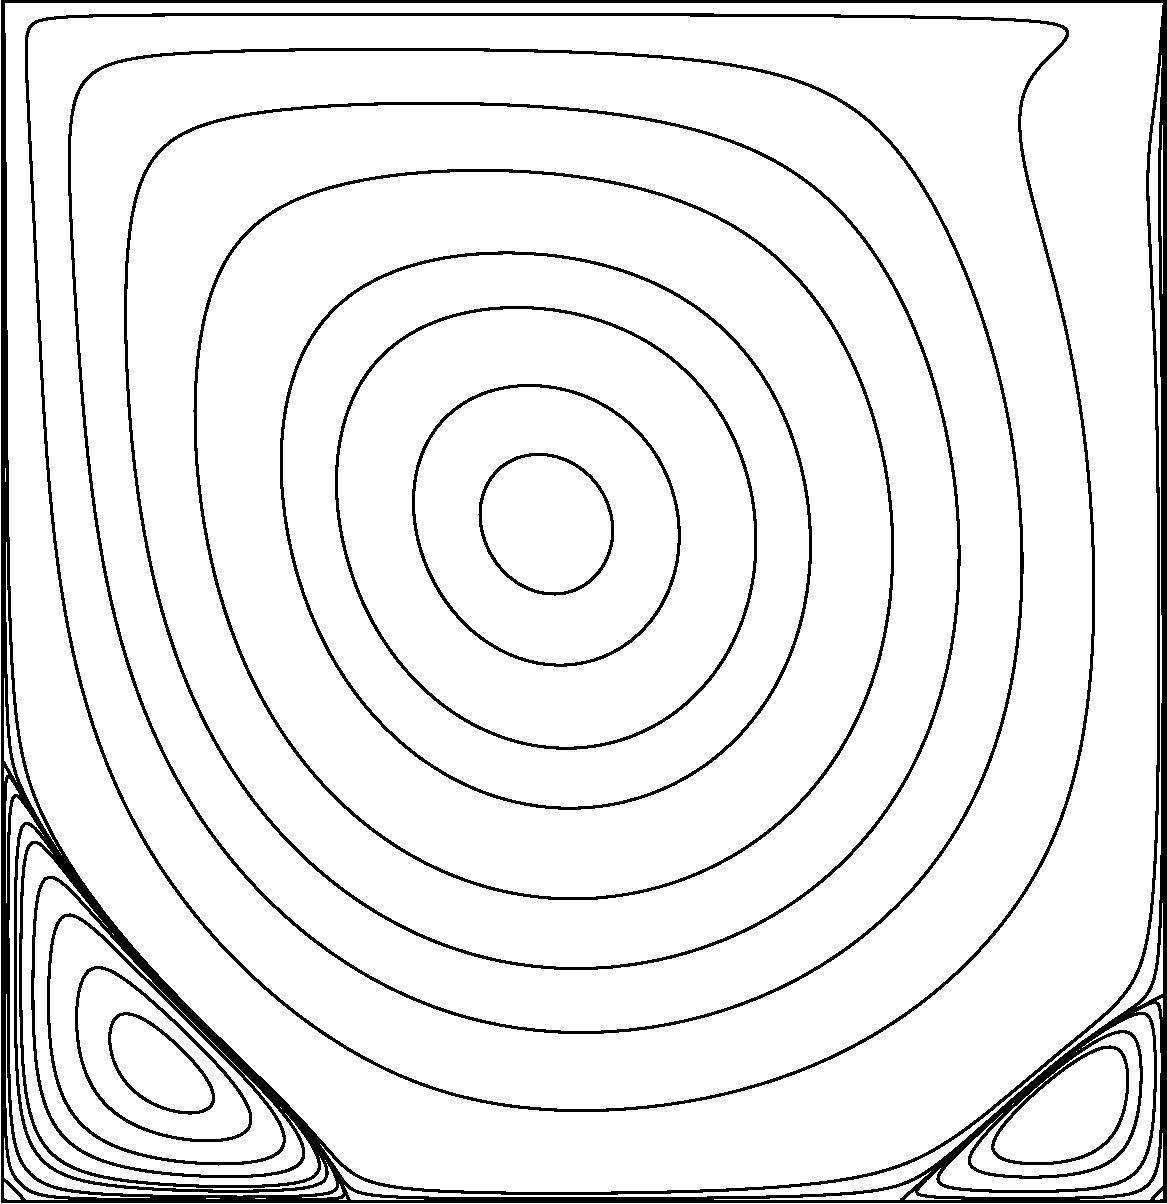
\includegraphics[width=0.85\textwidth]{Images/streamFunction.pdf}
    \caption{Stream function for $N = 64$, $\text{Re} = 1000$, $\Delta t = 0.0002$, and $\text{tol} = 1 \cdot 10^{-5}$.}
    \label{fig:SFN64}
\end{figure}

\begin{figure}[p]
    \centering
    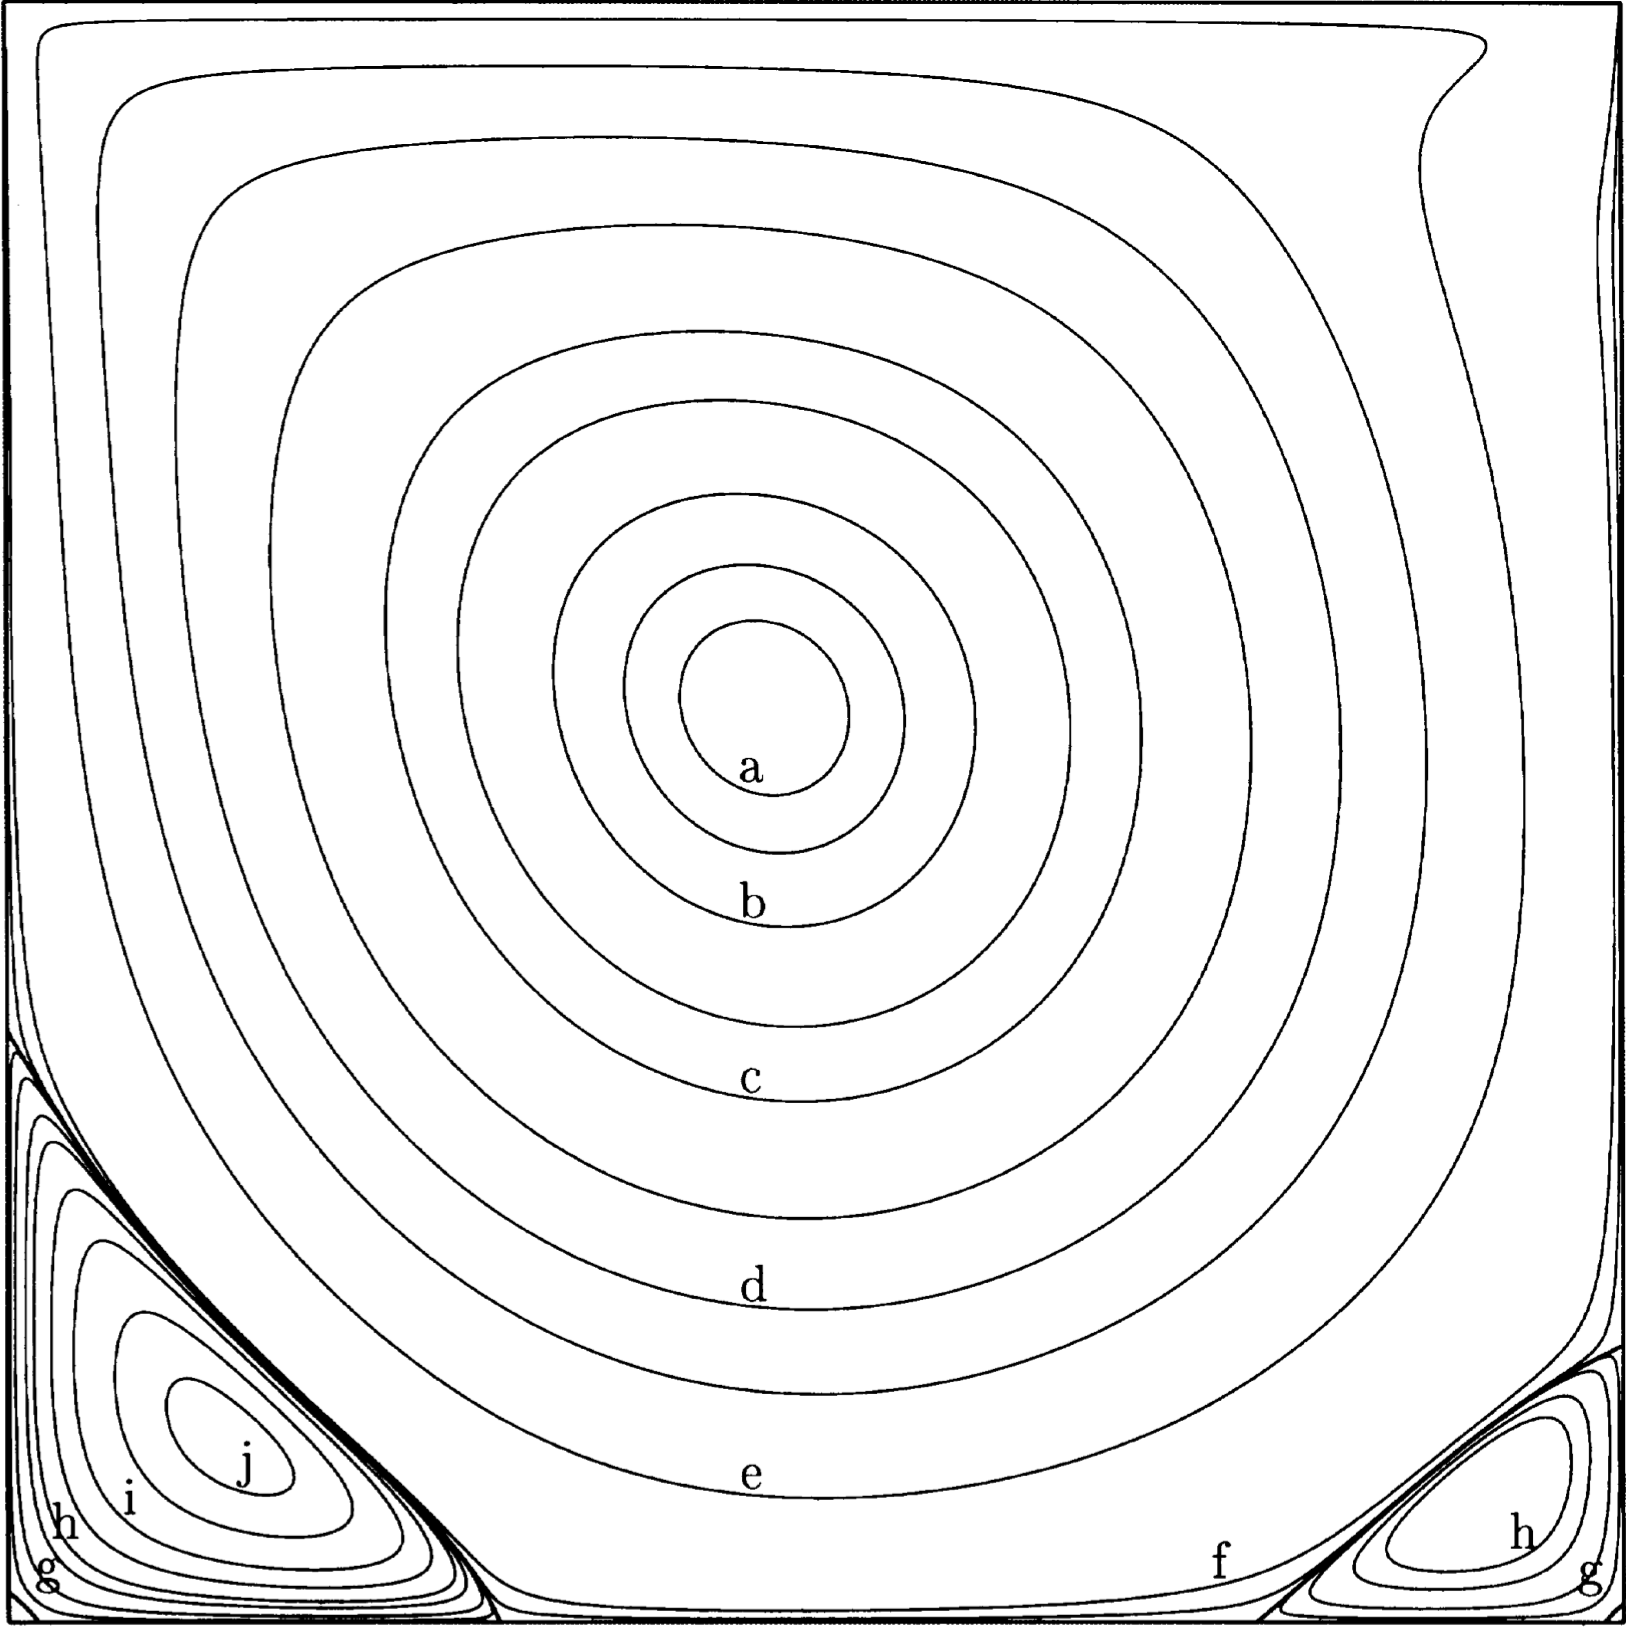
\includegraphics[width=0.85\textwidth]{Images/streamFunction.png}
    \caption{Benchmark stream function for $\text{Re} = 1000$ \parencite{botella1998benchmark}.}
    \label{fig:benchmarkSFN64}
\end{figure}

\begin{figure}[p]
    \centering
    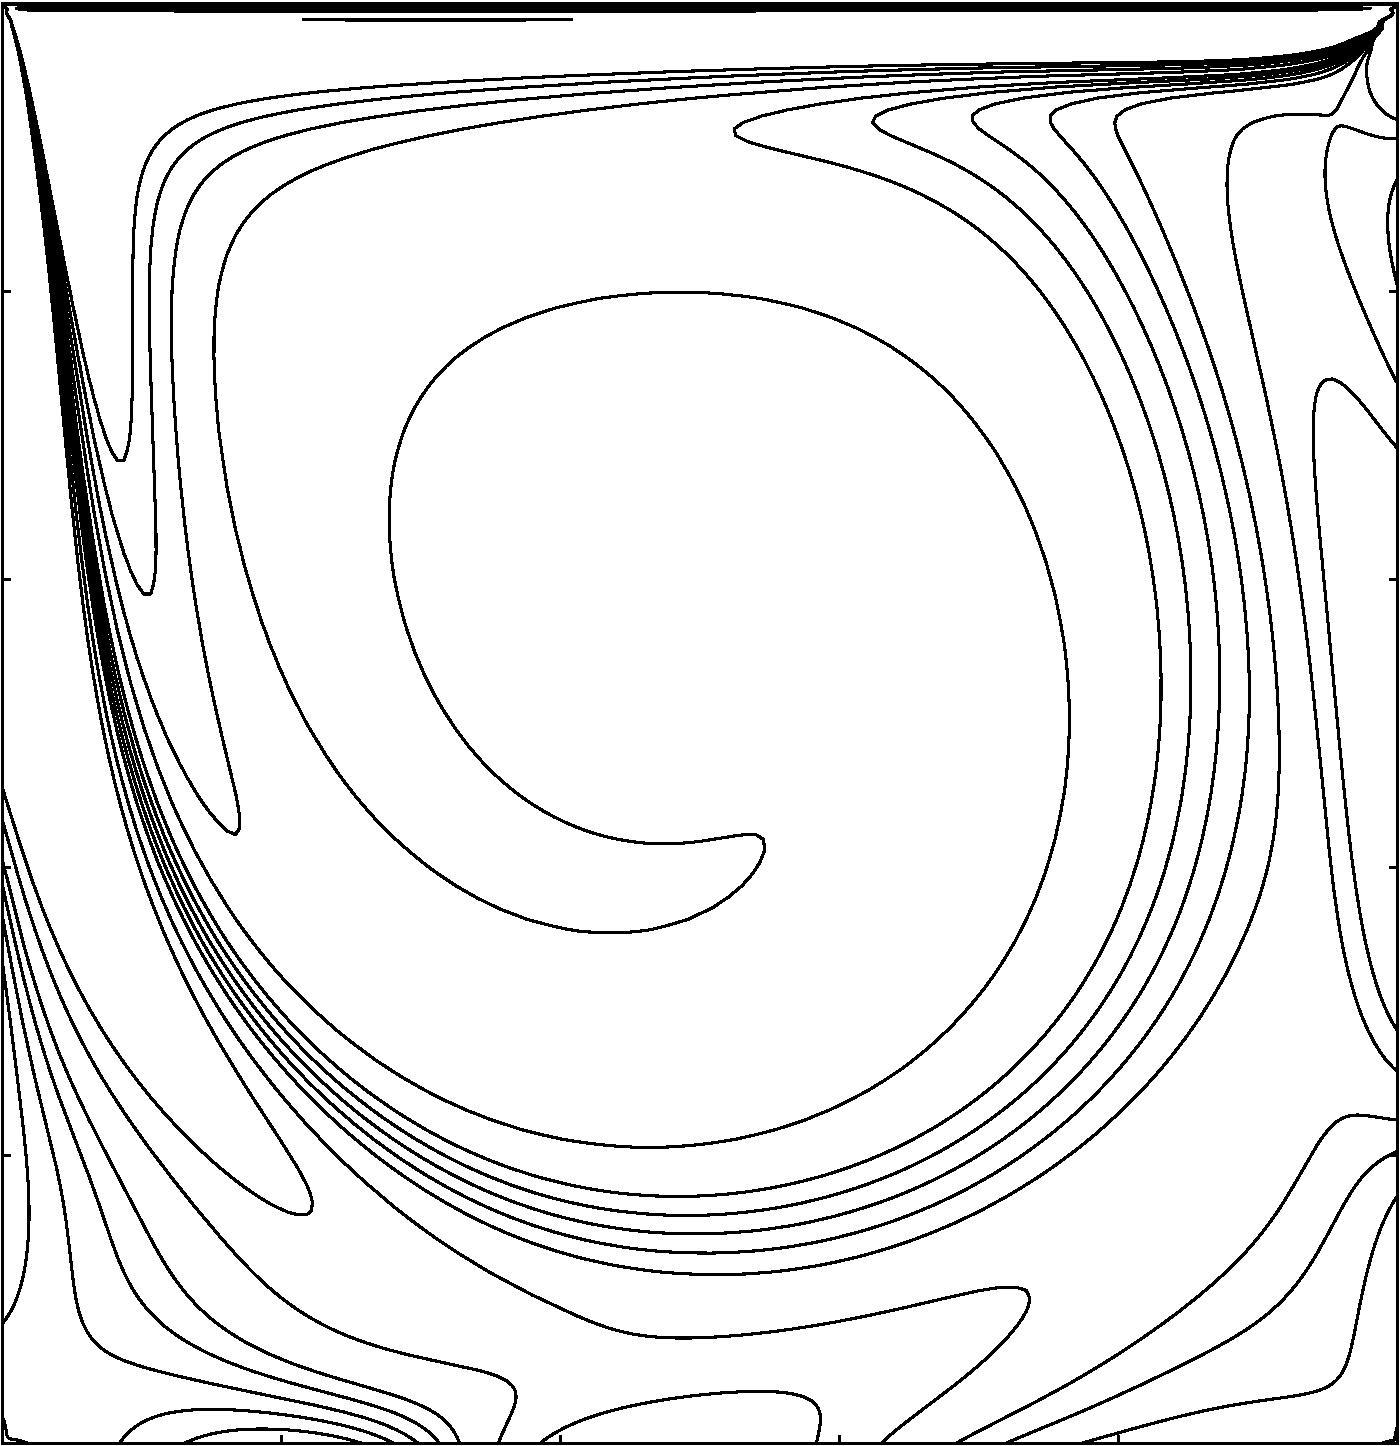
\includegraphics[width=0.85\textwidth]{Images/vorticity.pdf}
    \caption{Vorticity for $N = 64$, $\text{Re} = 1000$, $\Delta t = 0.0002$, and $\text{tol} = 1 \cdot 10^{-5}$.}
    \label{fig:VN64}
\end{figure}

\begin{figure}[p]
    \centering
    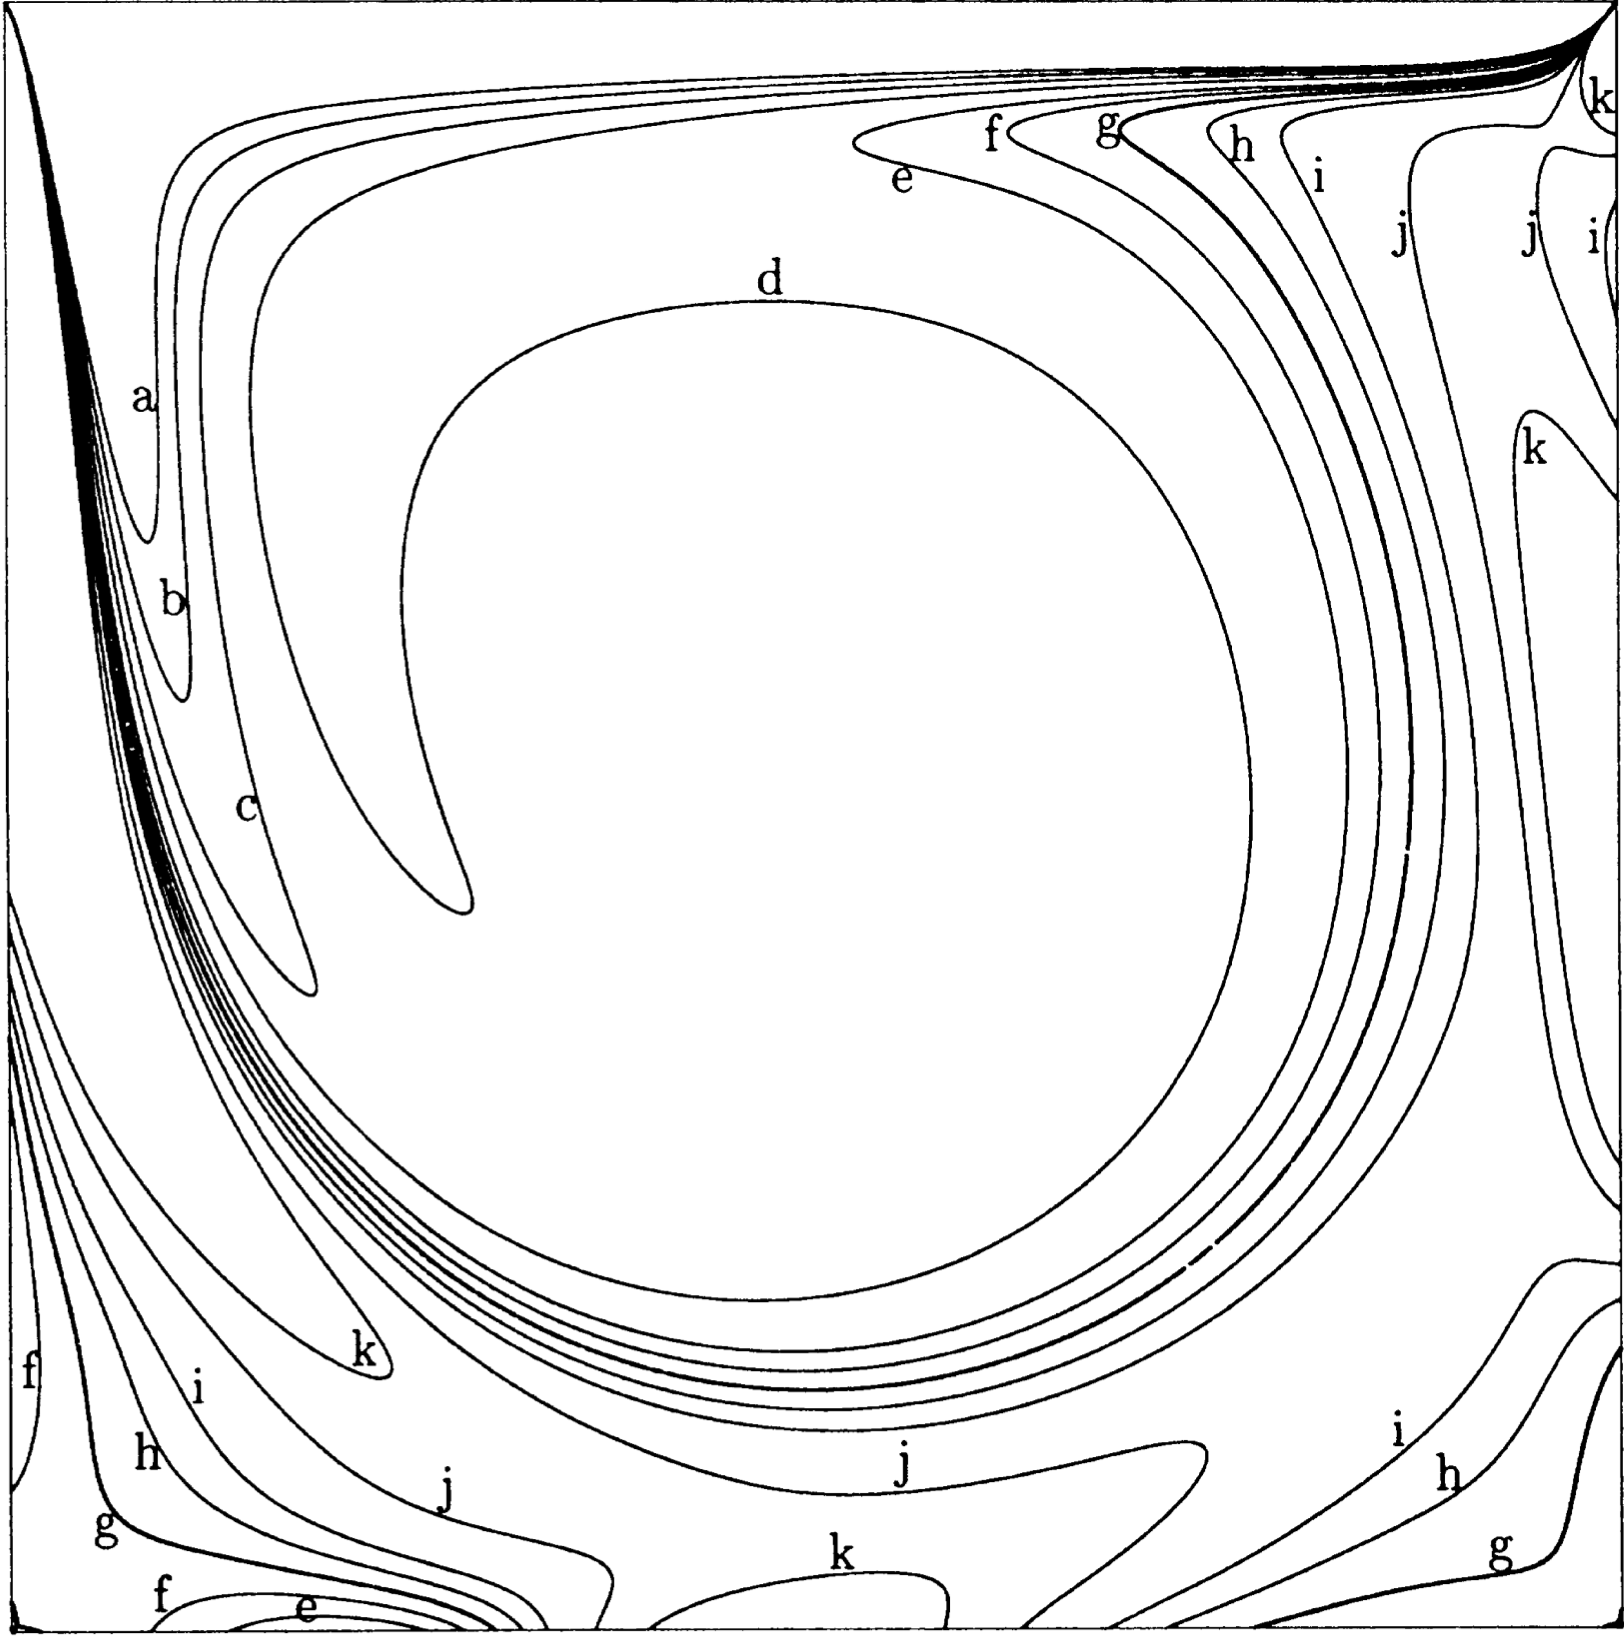
\includegraphics[width=0.85\textwidth]{Images/vorticity.png}
    \caption{Benchmark vorticity for $\text{Re} = 1000$ \parencite{botella1998benchmark}.}
    \label{fig:benchmarkVN64}
\end{figure}

\begin{figure}[p]
    \centering
    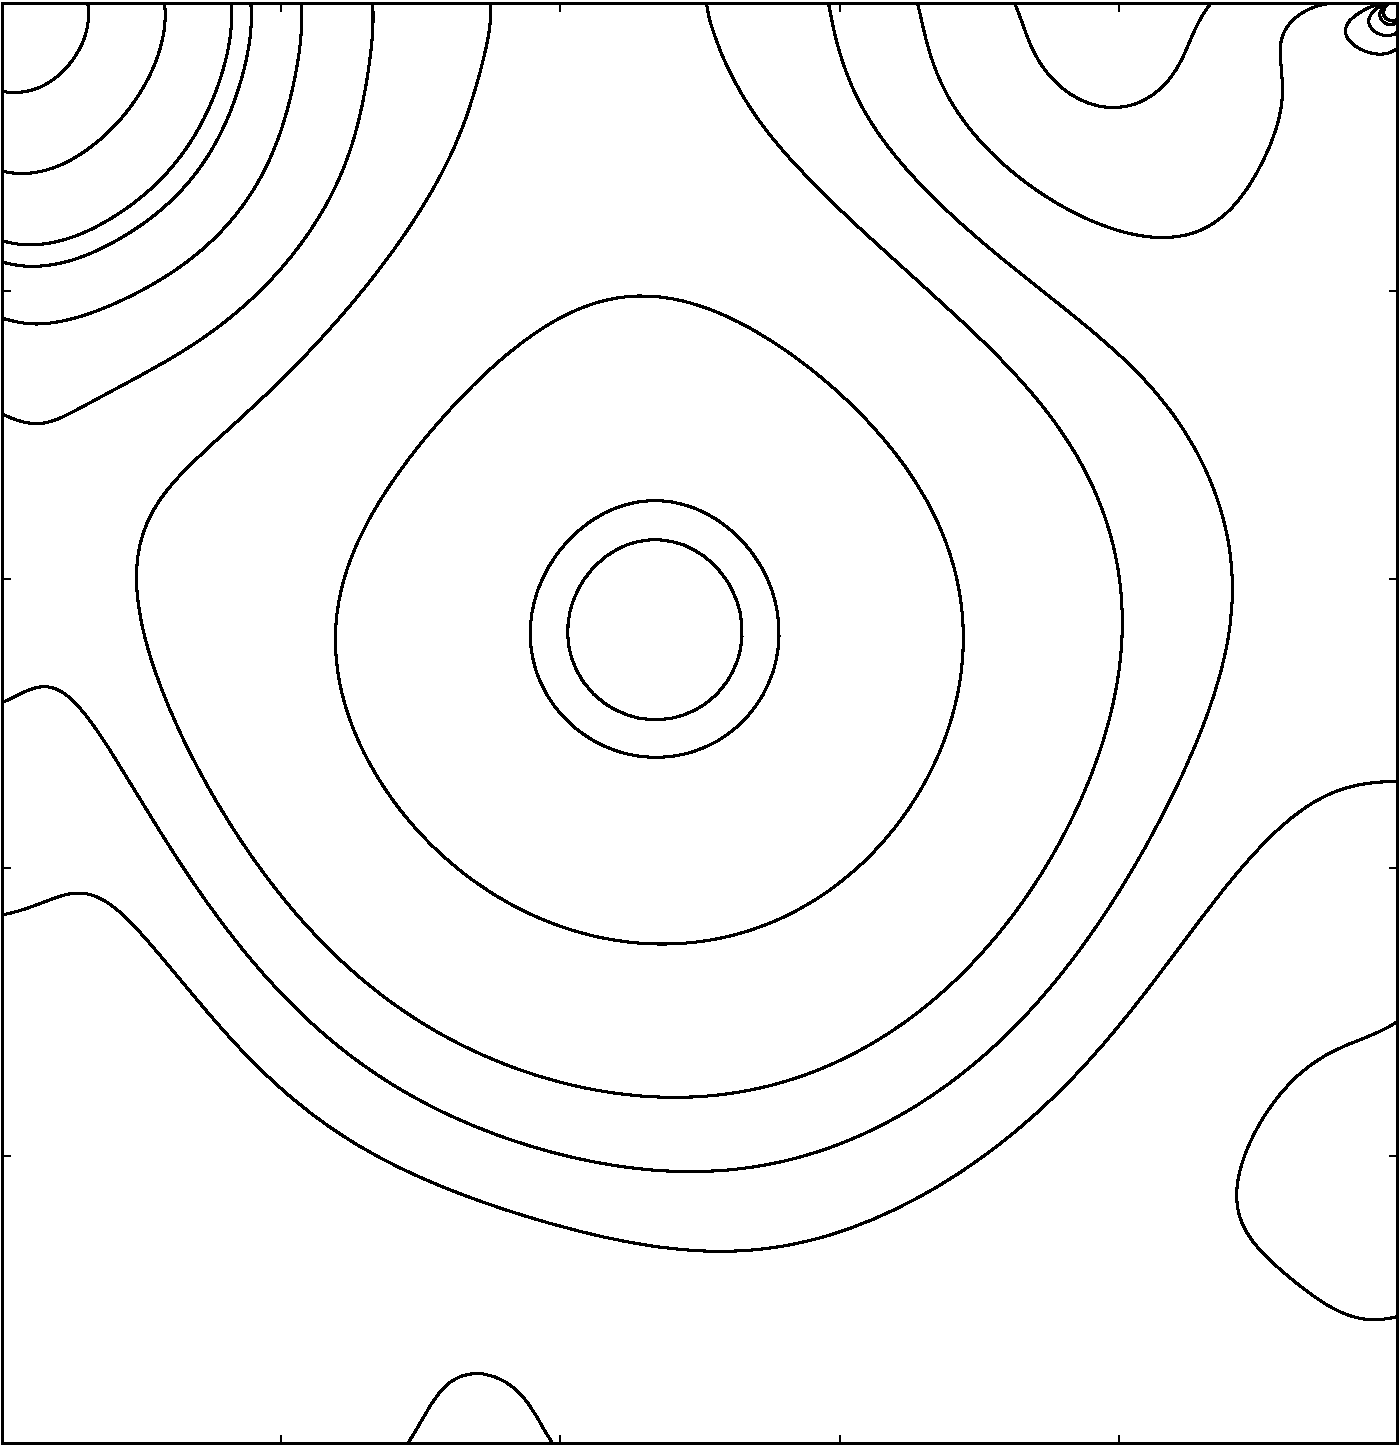
\includegraphics[width=0.85\textwidth]{Images/pressure.pdf}
    \caption{Pressure for $N = 64$, $\text{Re} = 1000$, $\Delta t = 0.0002$, and $\text{tol} = 1 \cdot 10^{-5}$.}
    \label{fig:PN64}
\end{figure}

\begin{figure}[p]
    \centering
    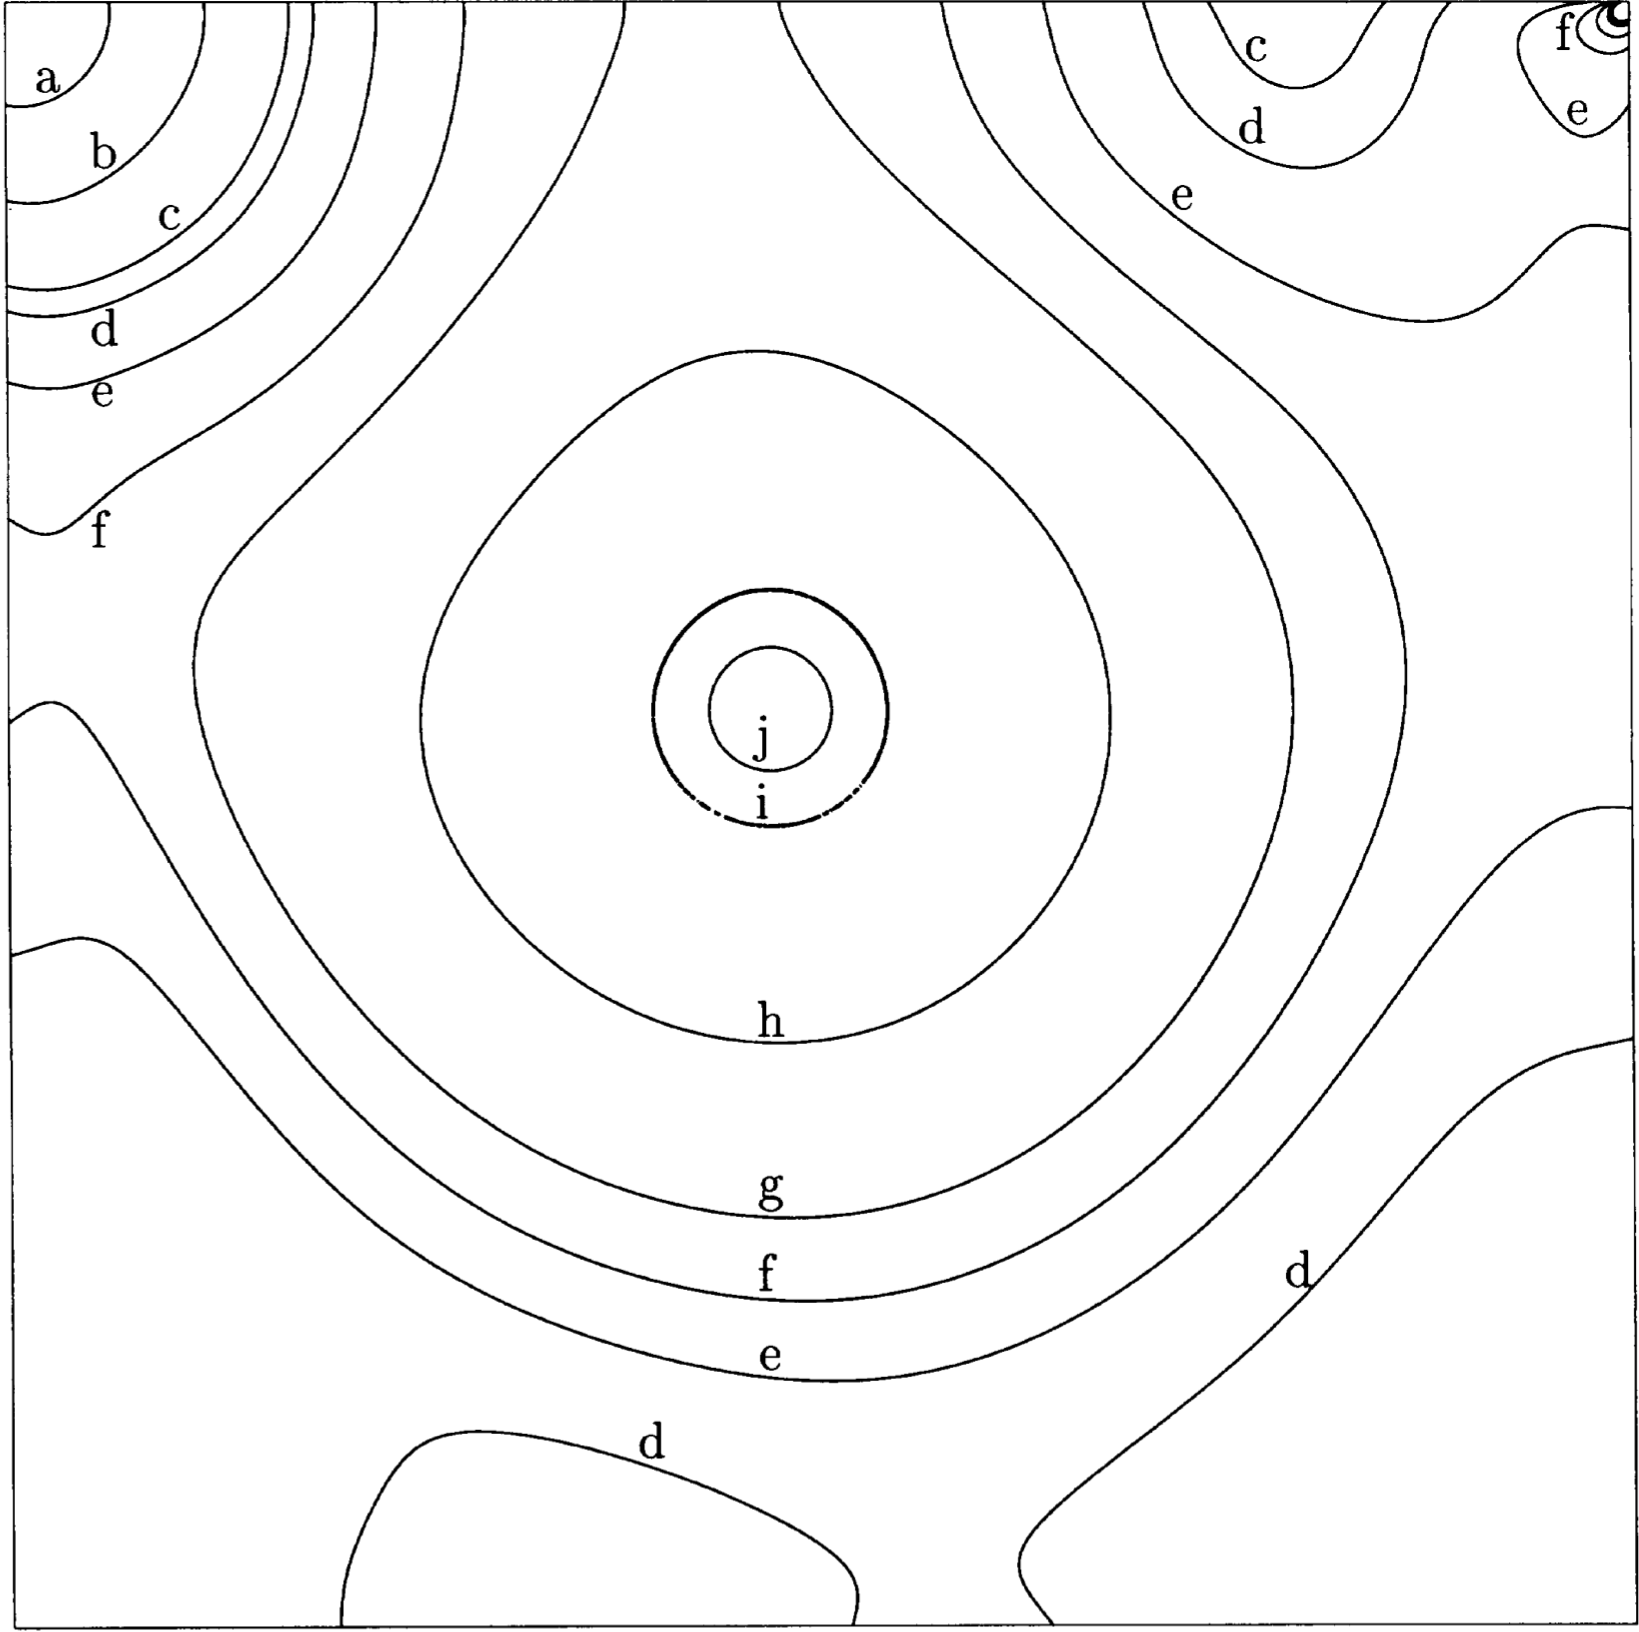
\includegraphics[width=0.85\textwidth]{Images/pressure.png}
    \caption{Benchmark pressure for $\text{Re} = 1000$ \parencite{botella1998benchmark}.}
    \label{fig:benchmarkPN64}
\end{figure}
